\documentclass[hidelinks,onefignum,onetabnum,final]{siamart220329}  % for arxiv
%\documentclass[review,hidelinks,onefignum,onetabnum,final]{siamart220329}  % for submission

\usepackage{amsfonts,yhmath}
\usepackage{graphicx}
\usepackage{epstopdf}
\ifpdf
  \DeclareGraphicsExtensions{.eps,.pdf,.png,.jpg}
\else
  \DeclareGraphicsExtensions{.eps}
\fi

% Used for creating new theorem and remark environments
\newsiamremark{remark}{Remark}
\newsiamremark{hypothesis}{Hypothesis}
\crefname{hypothesis}{Hypothesis}{Hypotheses}
\newsiamthm{claim}{Claim}
\newsiamremark{example}{Example}

\usepackage{amsopn}
\DeclareMathOperator{\diag}{diag}

\usepackage{bm,bbm,empheq,verbatim,fancyvrb,amssymb}
\usepackage{booktabs,multirow,xspace}
\usepackage{pifont}

\usepackage{tikz}
\usetikzlibrary{decorations.pathreplacing}
\usetikzlibrary{graphs,quotes}

\newcommand{\eps}{\epsilon}
\newcommand{\RR}{\mathbb{R}}

\newcommand{\grad}{\nabla}
\newcommand{\Div}{\nabla\cdot}

\newcommand{\bbf}{\mathbf{f}}
\newcommand{\bg}{\mathbf{g}}
\newcommand{\bn}{\mathbf{n}}
\newcommand{\bu}{\mathbf{u}}
\newcommand{\bw}{\mathbf{w}}
\newcommand{\bz}{\mathbf{z}}
\newcommand{\bX}{\mathbf{X}}

\newcommand{\bzero}{\bm{0}}

\newcommand{\btau}{\bm{\tau}}

\newcommand{\cB}{\mathcal{B}}
\newcommand{\cH}{\mathcal{H}}
\newcommand{\cK}{\mathcal{K}}
\newcommand{\cV}{\mathcal{V}}

\newcommand{\hcK}{\widehat{\cK}}

\newcommand{\nn}{{\text{n}}}
\newcommand{\pp}{{\text{p}}}

\newcommand{\ip}[2]{\left<#1,#2\right>}

\newcommand{\XX}{\ding{55}}

\newcommand{\dx}{\, \mathrm{d}x}

\newcommand{\rhoi}{\rho_{\text{i}}}

\DeclareMathOperator*{\argmin}{arg\,min}
\DeclareMathOperator*{\Hull}{Hull}


% running headers (as well as PDF metadata)
\headers{Bounds on geometry errors in glacier simulations}{E. Bueler}

\title{Bounds on geometry errors in glacier simulations}

\author{Ed Bueler\thanks{Department of Mathematics and Statistics, University of Alaska Fairbanks, USA (\email{elbueler@alaska.edu}).}}


\begin{document}
\maketitle

\begin{abstract}
The primary data which determine the evolution of glaciation are bedrock elevation and surface mass balance (snow accumulation minus melt).  From this data the glacier's geometry solves a free-boundary problem over a set of admissible surface elevation or thickness functions.  This constraint set requires that the ice surface elevation must be above the bedrock topography, equivalently that the ice thickness must be nonnegative.  For implicit time steps the free-boundary problem can be posed in weak form as a variational inequality over a fixed map-plane region.  We first show an abstract estimate for finite element approximations of such problems over Banach spaces, and in this estimate the nonlinear operator is assumed to be coercive and Lipshitz.  When applied in the glacier case, for which we must assume well-posedness of each continuous-space implicit time-step problem, certain terms in the finite element approximation can be further estimated.  The resulting computable bounds on the geometry approximation error are demonstrated in an implicit time-stepping glacier simulation based on non-shallow Stokes dynamics.
\end{abstract}

% REQUIRED
\begin{keywords}
error bounds, finite element methods, glaciers, ice flow, variational inequalities
\end{keywords}

% REQUIRED
%\begin{MSCcodes}
%FIXME
%\end{MSCcodes}


\section{Introduction} \label{sec:intro}

Glacier and ice sheet simulations typically model the ice layer as a free-surface, very-viscous, incompressible, and non-Newtonian fluid \cite{GreveBlatter2009,SchoofHewitt2013}.  For simplicity we will restrict our considerations to simulations of glaciers on land, without floating portions, and we note that an ``ice sheet'' is simply a continent-scale glacier.  Two types of essential input data into such simulations are the bedrock elevation (meters) and the surface mass balance (SMB).  We will assume that the bedrock elevations are constant in time.  By definition, the SMB is the annually-averaged difference of vertically-accumulating snow minus the loss of (liquid) water, through runoff, at the upper surface of the glacier \cite{Cogleyetal2011}.  The SMB is measured in ice-equivalent units of meters per second.

Thus a glacier simulation takes the topography and the changing climate as inputs.  Then, from an initial glacier geometry, it produces the glacier's evolving geometry and flow velocity; these are the output fields of primary scientific value.  The geometry is parameterized by a surface elevation or thickness function, measured in meters and depending on map-plane (two-dimensional) location and time.  The computed flow velocity is, however, only defined at those three-dimensional locations and times where ice is present.  Additional complications are common in models \cite{GreveBlatter2009}, including simulation of the internal energy of the ice \cite{Aschwandenetal2012}, and/or the presence of liquid water within the ice matrix or at the glacier surfaces.  However, here we consider only models which conserve mass and momentum, and which do not make shallowness assumptions, while conservation of energy is not addressed.

At a map-plane location and time where a glacier exists the surface elevation exceeds the bedrock elevation, equivalently the ice thickness is positive.  In other words, whether parameterized using surface elevation or thickness, the glacier's geometry must satisfy an inequality so as to be admissible, and so the mathematical models under consideration are inequality-constrained flow equations \cite{Bueler2021conservation}.  In fact, let $\Omega \subset \RR^2$ be a fixed portion of the earth's surface on which we are interested in glaciation (Figure \ref{fig:stokesdomain}).  Let $x\in\Omega$ denote the map-plane coordinate(s).  Assume we are given, as data, a bed elevation function $b(x)$ and an SMB function $a(t,x)$ for $t\in [0,T]$ and $x\in \Omega$.  (Function spaces for these data will be considered below.)  Note that $a$ is generally signed.  In areas where $a>0$ (accumulation; draw as downward arrows in Figure \ref{fig:stokesdomain}) then a glacier will exist, but if $a<0$ (upward arrows) then either a glacier exists with an ablating surface, or no glacier exists.  Determining which situation applies requires solving a free-boundary problem.

\medskip
\begin{figure}[ht]
\centering
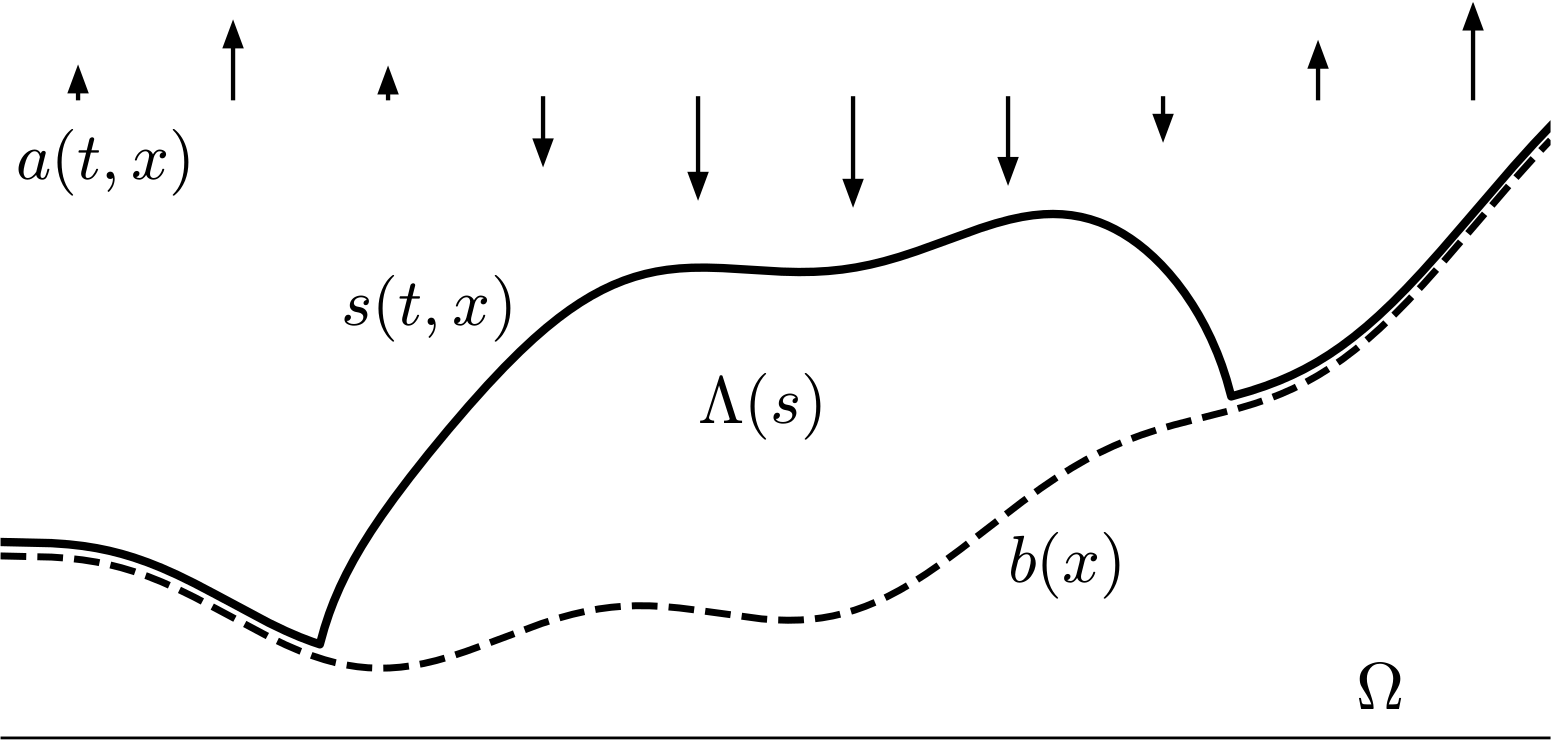
\includegraphics[width=0.65\textwidth]{genfigs/stokesdomain.pdf}
\caption{Glacier geometry notation used in this paper.}
\label{fig:stokesdomain}
\end{figure}

\medskip
Let $s(t,x)$ be the (solution) ice surface elevation.  We will regard this as defined everywhere, but subject to the constraint that the surface $z=s(t,x)$ must be at or above the bedrock: $s(t,x) \ge b(x)$.  The solution ice velocity $\bu(t,x,z)$ and pressure $p(t,x,z)$ are then defined only on the domain
\begin{equation}
\Lambda(t) = \left\{(x,z)\,:\,b(x) < z < s(t,x)\right\} \subset \Omega \times \RR \subset \RR^3. \label{eq:icydomain}
\end{equation}
It is important to emphasize this aspect of glacier models: at any time $t$ the 3D domain $\Lambda(t)$, on which the velocity and pressure are meaningful, is determined by the time-dependent surface elevation $s(t,x)$, which is also part of the solution.  Some regions in $\Omega$ may have no ice at all ($s(t,x)=b(x)$).

Denote the surface value (trace \cite{Evans2010}) of the velocity solution by $\bu|_s$, and let $\bn_s = \left<-\grad s,1\right>$ be a 3D, un-normalized surface normal vector.  For any $T>0$, an infinite-dimensional nonlinear complementarity problem (NCP) \cite{Bueler2021conservation,FacchineiPang2003,SchoofHewitt2013} applies almost everywhere in $[0,T]\times \Omega$:
\begin{subequations}
\label{eq:ncp}
\begin{align}
s - b &\ge 0 \\
\frac{\partial s}{\partial t} - \bu|_s \cdot \bn_s - a &\ge 0 \\
(s - b) \left(\frac{\partial s}{\partial t} - \bu|_s \cdot \bn_s - a\right) &= 0
\end{align}
\end{subequations}
This strong form NCP statement, which will be reformulated as a variational inequality (VI; \cite{KinderlehrerStampacchia1980}) in Section \ref{sec:models}, assumes the extension $\bu|_s=0$  to the ice-free areas where $s(t,x)=b(x)$.

From \eqref{eq:ncp}, at a given map-plane location and time either no glacier is present ($s=b$) or the surface kinematical equation (SKE) holds:
\begin{equation}
\frac{\partial s}{\partial t} - \bu|_s \cdot \bn_s - a = 0.  \label{eq:ske}
\end{equation}
This well-known equation \cite{SchoofHewitt2013} states that the non-material surface of the ice moves vertically according to the sum of a component of the ice velocity, at the ice surface, and the SMB.  It is a statement of mass conservation at a non-material surface \cite{Aschwandenetal2012}, sometimes wrongly\footnote{Equation \eqref{eq:ske} is not the boundary condition for any identifiable problem.} called a ``kinematical boundary condition'' \cite{GreveBlatter2009}.

Within the ice the simulation will conserve mass and momentum.  Recalling \eqref{eq:icydomain}, let $\Gamma_s(t) \subset \partial \Lambda(t)$ be the upper surface $z=s$ and
$\Gamma_b(t) \subset \partial \Lambda(t)$ be the base $z=b$.  The models considered here neglect the possibility of fracture-generated cliffs at the ice margin, and we assume $\partial \Lambda(t) = \Gamma_s(t) \cup \Gamma_b(t)$ at any time.  (Compare the well-posedness considerations at the end of Section \ref{sec:models}.)  The standard non-shallow model is then a non-Newtonian Stokes problem \cite{GreveBlatter2009,JouvetRappaz2011,SchoofHewitt2013} over $\Lambda(t)$, wherein
\begin{equation}
\nu(D\bu) = \frac{\Gamma}{2} |D\bu|^{\pp-2} \label{eq:glen}
\end{equation}
defines the ice viscosity according to Glen's power law \cite{GreveBlatter2009}, and $D\bu=\frac{1}{2}(\grad \bu + \grad \bu^{\top})$ denotes the strain rate tensor.  The exponent $\pp$, often written $\pp=\nn+1$ in glaciology \cite{GoldsbyKohlstedt2001}, is approximately 4.  (Note $\pp=2$ yields a Newtonian fluid.)  The coefficient $\Gamma>0$ is determined by the measured properties of ice \cite{GoldsbyKohlstedt2001,GreveBlatter2009}, but we assume it to be constant, modeling an isothermal situation.

If $\rhoi$ is the density of ice and $\bg$ is the acceleration of gravity then the Stokes problem for a glacier with nonsliding (e.g.~frozen) base \cite{JouvetRappaz2011} is
\begin{subequations}
\label{eq:stokes}
\begin{align}
- \nabla \cdot \left(2 \nu(D\bu)\, D\bu\right) + \nabla p - \rhoi \bg &= \bzero && \text{within $\Lambda(t) \subset \RR^3$} \\
\nabla \cdot \bu &= 0 && \text{within $\Lambda(t) \subset \RR^3$} \label{eq:stokes:incomp} \\
\left(2 \nu(D\bu) D\bu - pI\right) \bn_s &= \bzero && \text{on $\Gamma_s(t)$}\label{eq:stokes:stressfreesurface} \\
\bu  &= 0 && \text{on $\Gamma_b(t)$}
\end{align}
\end{subequations}
Equation \eqref{eq:stokes:incomp} states incompressibility and \eqref{eq:stokes:stressfreesurface} that the sub-aerial upper surface is stress free; \eqref{eq:stokes:stressfreesurface} should not be confused with \eqref{eq:ske}.

In summary at this point, a glacier simulation is an evolving free-surface flow, subject to a signed climate (i.e.~SMB) that can add or remove ice, coupled to a Stokes problem within an evolving, 3D icy domain.  The evolution of the solution variables $s(t,x)$, $\bu(t,x,z)$, and $p(t,x,z)$ is found from an initial surface elevation $s(0,x)$ and the data $b(x),a(t,x)$.  The surface elevation $s(t,x)$ is defined everywhere, i.e.~over $[0,T]\times \Omega$, but it is subject to $s(t,x) \ge b(x)$.

The surface elevation $s(t,x)$ and surface velocity $\bu|_s(t,x)=\bu(t,x,s(t,x))$ are linked by the kinematical NCP \eqref{eq:ncp}.  However, because the flow is very viscous \cite{Acheson1990}, the Stokes model \eqref{eq:stokes} acts as an instantaneous ``algebraic'' constraint on the evolution statement \eqref{eq:ncp}.  The coupled, infinite-dimensional system \eqref{eq:icydomain}--\eqref{eq:stokes} is therefore both a differential algebraic equation (DAE) system \cite{AscherPetzold1998} and an NCP.

Glacier simulations are commonly formulated using a finite element (FE) method for the Stokes sub-problem \cite{IsaacStadlerGhattas2015,Jouvetetal2008,Pattynetal2008}, or for a shallow approximation thereof.  However, to the author's knowledge all existing non-shallow (Stokes) evolution models use a explicit time-stepping scheme for the geometry, for example as in \cite{Jouvetetal2008} or \cite{LofgrenAhlkronaHelanow2022}, with the one exception of the work \cite{WirbelJarosch2020}.

Each time step of these models will have a variational inequality (VI) weak formulation \cite{Evans2010,KinderlehrerStampacchia1980}.  We must choose whether glacier geometry in this formulation is parameterized by surface elevation or thickness.  While equivalent in the continuum problem, the two formulations have different character when FE approximations are applied, and in the abstract estimate of Section \ref{sec:abstractestimate}.  Surface elevation $s(t,x)$ is preferred because of the flow-caused smoothing effect illustrated in Figure \ref{fig:giscross}.  For land-based glaciers $s(t,x)$ is smoother in $x$ than is the thickness $H(t,x) = s(t,x)-b(x)$ because the latter ``inherits'' the lower regularity of the eroded and faulted bedrock topography.

\begin{figure}
\begin{minipage}[t]{0.85\textwidth}
\vspace{0pt}
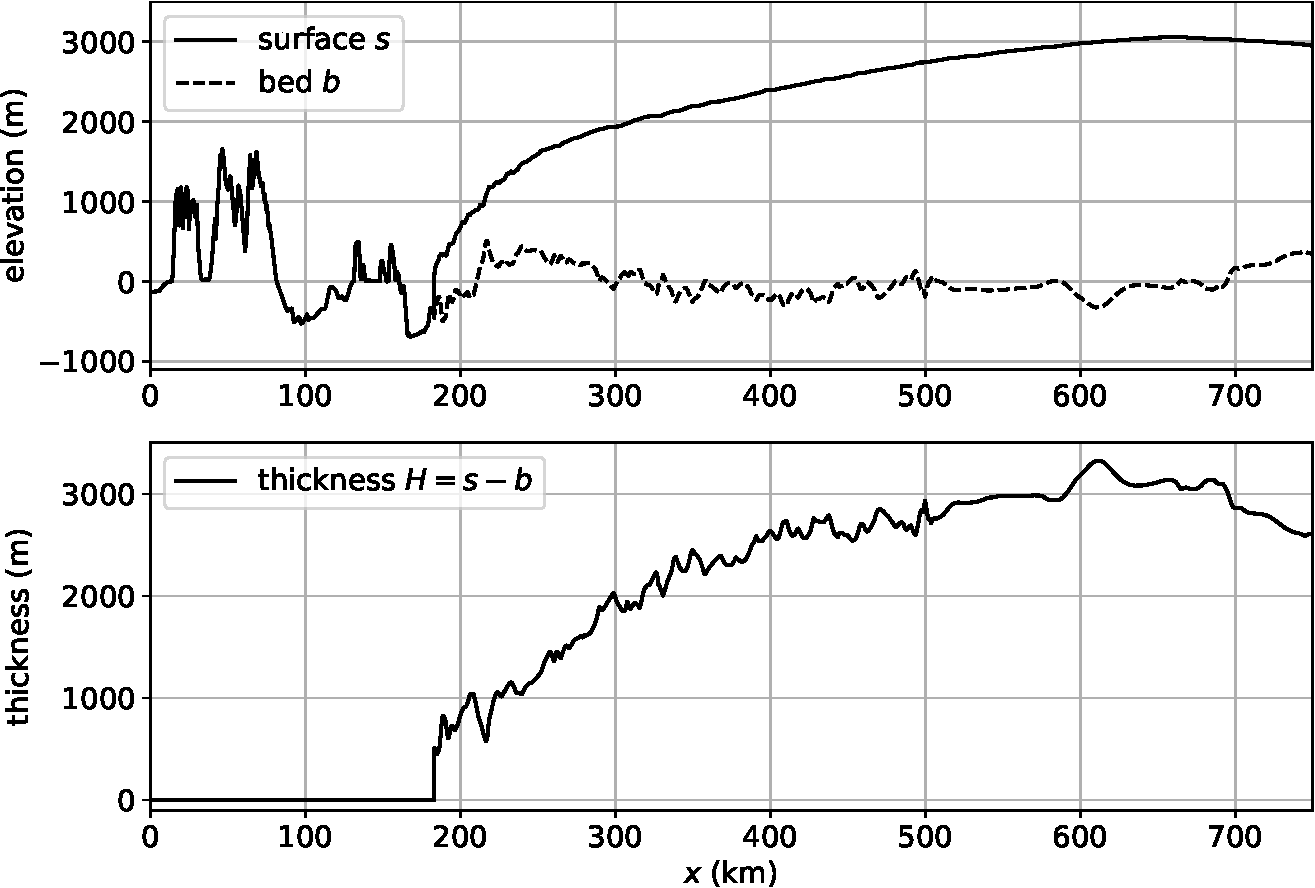
\includegraphics[width=\textwidth]{genfigs/giscross.pdf}
\end{minipage}
\,
\begin{minipage}[t]{0.13\textwidth}
\vspace{10pt}
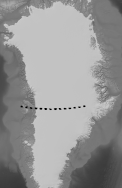
\includegraphics[width=\textwidth]{genfigs/gis/gris-profile-gray.png}
\end{minipage}
\caption{A cross-section of the Greenland ice sheet at $70^\circ$N latitude (inset).  While the ice surface $s$ is relatively smooth because of ice flow (top), the bedrock elevation $b$ is much rougher.  The corresponding ice thickness $H = s-b$ (bottom), though it is a valid description of glacier geometry, inherits the low regularity of $b$.  (Data from \cite{Morlighemetal2017} and A.~Aschwanden, personal communication.)}
\label{fig:giscross}
\end{figure}

FIXME: WHAT WE ACCOMPLISH

This paper is organized as follows.  In Section \ref{sec:models} we reformulate the coupled problem \eqref{eq:icydomain}--\eqref{eq:stokes} as a VI weak form for (implicit) backward Euler time steps.  Well-posedness for this time-step problem is conjectured, over a Banach space of surface elevation functions.  (The thickness function version is also stated.)  Then in Section \ref{sec:abstractestimate} we show an abstract FE error estimate (Theorem \ref{thm:abstractestimate} and its corollaries) for general VI problems involving fully-nonlinear, but coercive and Lipshitz, operators on Banach spaces.  This estimate extends the classical bilinear, elliptic case by Falk \cite{Falk1974}.  In Section \ref{sec:application} we apply this theorem to the glacier time steps from Section \ref{sec:models}.  The distinctive character of how glaciers respond to climate implies that certain terms are effectively small.  A set of computable geometry error estimates is proposed.  These estimates are demonstrated in Section \ref{sec:demo} on an idealized, but non-trivial, glacier simulation implemented in Firedrake \cite{Hametal2023}.


\section{Implicit time-stepping variational inequality models} \label{sec:models}

As in the Introduction, let $\Omega \subset \RR^2$ be a fixed region of land, suppose $b \in C^1(\Omega)$ is the time-independent bedrock elevation on $\Omega$, and, for $T>0$, let $a(t,x) \in C([0,T] \times \Omega)$ be the given surface mass balance (SMB) function.  Where $a(t,x)>0$ there is more snow in a year than can melt (accumulation), while if $a(t,x)<0$ the opposite is true (ablation).  Note that $a(t,x)$ is assumed to be defined everywhere in $\Omega$, regardless of whether a glacier is present or not, though necessarily $a(t,x) \le 0$ where there is no glacier.  At such an ablative location the value of $a(t,x)$ can be modeled using knowledge of precipitation plus an energy balance \cite{GreveBlatter2009}.  For example, one may hypothesize an ice or snow surface and then compute the total runoff from the available energy for melt, and then balance this against snow accumulation, if any.  In any case, in a well-posed glacier geometry evolution model, $a(t,x)$ at an unglaciated location will be the SMB which a glacier would experience if it were present at that time and place.

Recall the surface kinematical equation (SKE) \eqref{eq:ske}, and the nonlinear complementarity problem (NCP) \eqref{eq:ncp} in which it appears.  Let $\{t_n\}$ be an increasing sequence of times, and write $s(x) = s^n(x)\approx s(t_n,x)$ for the unknown surface elevation at time $t_n$.  Using a backward Euler implicit step \cite{AscherPetzold1998}, \eqref{eq:ske} is approximated by
\begin{equation}
\frac{s - s^{n-1}}{\Delta t} - \bu|_s \cdot \bn_s - a^n = 0. \label{eq:be:ske}
\end{equation}
where $\Delta t = t_n-t_{n-1}$ and $s^{n-1}(x) \approx s(t_{n-1},x)$.  For the SMB term $a^n$, assume that a temporal average has been computed.  Equivalently, let
\begin{equation}
\ell^n(x) = s^{n-1}(x) + \int_{t_{n-1}}^{t_n} a(t,x)\,dt, \label{eq:be:source}
\end{equation}
so that $\ell^n=s^{n-1}+\Delta t\,a^n$.  The computable function $\ell^n$, which would be the updated surface elevation in the absence of flow, is a source term in what follows.

The implicit step solution $s$ will not generally solve \eqref{eq:be:ske} in all of $\Omega$.  Instead, similar to \eqref{eq:ncp}, an NCP holds:
\begin{subequations}
\label{eq:be:ncp}
\begin{align}
s - b &\ge 0 \label{eq:be:ncp:constraint} \\
s - \Delta t\,\bu|_s \cdot \bn_s - \ell^n &\ge 0 \\
(s - b) \left(s - \Delta t\,\bu|_s \cdot \bn_s - \ell^n\right) &= 0
\end{align}
\end{subequations}

The strong form NCP \eqref{eq:be:ncp} has a weak form VI version which is suited to finite element (FE) approximation.  To state it we must hypothesize that surface elevations are in a Banach space $\cV$ of real-valued functions on $\Omega$.  (The precise space is unknown, but we will say more about it later in this Section.)  The admissible surface elevations are those which are above the bed, which defines a convex and closed subset:
\begin{equation}
\cK = \left\{r \in\cV\,:\,r \ge b\right\} \subset \cV.  \label{eq:be:admissible}
\end{equation}

To derive the VI form suppose $s$ is continuous and otherwise sufficiently regular so as to solve NCP \eqref{eq:be:ncp}.  The following argument is from \cite{Bueler2021conservation}.  Let $I$ be a measurable subset of $\Omega$ on which constraint \eqref{eq:be:ncp:constraint} is inactive, so a glacier is present on $I$: $I \subset \{x\,:\,s(x)>b(x)\}$.    Then, because \eqref{eq:be:ske} holds on all of $I$, it follows by integration that
\begin{equation}
\int_I \left(s - \Delta t\,\bu|_s \cdot \bn_s - \ell^n\right)\,(r-s) = 0.
\end{equation}
for all $r\in\cK$.  On the other hand, suppose $A \subset \Omega$ is measurable and a subset of the active region, i.e.~$A$ is in the ice-free region: $A \subset \{x\,:\,s(x)=b(x)\}$.  Note that $r-s=r-b\ge 0$ on $A$ for $r\in\cK$.  In this case we observe that $\ell^n - b = s^{n-1} - b + \Delta t\,a^n\le 0$ on all of $A$ because otherwise, using the continuity of $b$, $s^{n-1}$, and $a^n$, a glacier would still be present, or would have appeared, somewhere in $A$, a contradiction.  Using $\bu|_s=0$ on $A$, i.e.~extension by zero, integration then shows an inequality because $b-\ell^n \ge 0$ and $r-s\ge 0$ on $A$:
\begin{equation}
\int_A \left(s - \Delta t\,\bu|_s \cdot \bn_s - \ell^n\right)\,(r-s) = \int_A \left(b - \ell^n\right)\,(r-b) \ge 0.
\end{equation}

Since almost all parts of $\Omega$ are either covered by glacier (in $I$) or ice free (in $A$), the argument above justifies the following VI model for the implicit time step solution surface elevation $s \in \cK$:
\begin{equation}
\int_\Omega \left(s - \Delta t\,\bu|_s \cdot \bn_s\right)\,(r-s) \ge \int_\Omega \ell^n \,(r-s) \quad \text{for all } r \in \cK. \label{eq:be:viearly}
\end{equation}
	
FIXME however we need to solve Stokes equations on $\Lambda(t)$ to get $\bu|_s$; here is weak form for that
\begin{equation}
XX \text{(see \cite{JouvetRappaz2011}, \cite{IsaacStadlerGhattas2015})} \label{eq:be:stokes}
\end{equation}
this is well posed \cite{JouvetRappaz2011}

FIXME now let
\begin{equation}
F(s) = s - \Delta t\,\Phi(s) \cdot \bn_s  \label{eq:be:Fdefine}
\end{equation}
and
\begin{equation}
\Phi(s) = \left(\text{trace of the solution $\bu$ of \eqref{eq:be:stokes} along upper surface $\Gamma_s$}\right)  \label{eq:be:Phidefine}
\end{equation}

FIXME restate VI: seek $s = s^n \in \cK$ so that 
\begin{equation}
\int_\Omega F(s)\,(r-s) \ge \int_\Omega \ell^n \,(r-s) \quad \text{for all } r \in \cK. \label{eq:be:vi}
\end{equation}

FIXME conjecture well-posedness of \eqref{eq:be:vi} for sufficiently short $\Delta t$

FIXME VI for mass continuity with $H$: fluid layer thickness equation, also called mass continuity or Saint Venant equation \cite{JouvetBueler2012}, $\cK = \{H\ge 0\}$, $\cK_h \subset \cK$, apparently $\eta = H^{2p/(p-1)} \in W^{1,p}(\Omega)$, for e.g.~$p=4$, because of existence in SIA case \cite{JouvetBueler2012}

FIXME SIA model has better-known properties \cite{JouvetBueler2012,PiersantiTemam2023}. however, regularity arising from analyzing SIA is not to be trusted because non-shallow (Stokes) dynamics is not diffusive for short wavelength surface/thickness perturbations \cite{Pattynetal2008}


\section{Abstract error estimate} \label{sec:abstractestimate}

We first consider an abstract variational inequality (VI) \cite{KinderlehrerStampacchia1980} problem as follows.  Let $\cV$ be a real reflexive Banach space with norm $\|\cdot\|$ and topological dual space $\cV'$.  Denote the dual pairing of $\phi \in \cV'$ and $v\in\cV$ by $\ip{\phi}{v} = \phi(v)$, and define the (Banach space) norm on $\cV'$ by $\|\phi\|_{\cV'} = \sup_{\|v\|=1} |\!\ip{\phi}{v}\!|$.

Let $\cK \subset \cV$ be a nonempty, closed, and convex subset, called the constraint set.  Elements of $\cK$ are said to be admissible.  For a continuous, but generally nonlinear, operator $f:\cK \to \cV'$, and a linear source $\ell\in \cV'$, the VI problem is to find $u\in \cK$ such that
\begin{equation}
\ip{f(u)}{v-u} \ge \ip{\ell}{v-u} \quad \text{for all } v\in \cK. \label{eq:vi}
\end{equation}
The best know example of \eqref{eq:vi} is the obstacle problem for the Laplacian operator; see e.g.~subsections 5.1 in \cite{Ciarlet2002} or 8.4.2 in \cite{Evans2010}.

\begin{definition} \label{def:monotonepcoercive}
An operator $f:\cK \to \cV'$ is said to be \emph{monotone} if
\begin{equation}
\ip{f(v)-f(w)}{v-w} \ge 0 \qquad \text{for all } v,w \in \cK \label{eq:monotone}
\end{equation}
and \emph{strictly monotone} if equality in \eqref{eq:monotone} implies $u=v$ \cite{KinderlehrerStampacchia1980}.  Let $p>1$.  The operator is \emph{$p$-coercive} \cite{Bueler2021conservation} if there exists $\alpha>0$ such that
\begin{equation}
\ip{f(v)-f(w)}{v-w} \ge \alpha \|v-w\|^p \qquad \text{for all } v,w \in \cK. \label{eq:pcoercive}
\end{equation}
\end{definition}

Clearly, if $f$ is $p$-coercive then it is monotone and strictly monotone, in which case any solution of \eqref{eq:vi} is unique.  Furthermore, it is well-known that if $f:\cK \to \cV'$ is also continuous on finite-dimensional subspaces then VI \eqref{eq:vi} has a solution \cite[Corollary III.1.8]{KinderlehrerStampacchia1980}.  Thus $p$-coercivity and appropriate continuity of $f$ show well-posedness for \eqref{eq:vi}.

% \cite{Peral1997} uniform continuity over bounded sets for p-Laplacian: Thm A.0.6

\begin{definition} \label{def:lipshitz}
For $\rho>0$ let $B_\rho = \{v\in \cV\,:\,\|v\|\le \rho\}$.  We say $f:\cK \to \cV'$ is \emph{Lipshitz on bounded sets of $\cK$} if for every $\rho>0$ there is $C(\rho)>0$ so that if $v,w \in B_\rho \cap \cK$ and $z\in\cV$ then $|\ip{f(v)-f(w)}{z}| \le C(\rho) \|v-w\| \|z\|$.  Equivalently:
\begin{equation}
\|f(v)-f(w)\|_{\cV'} \le C(\rho) \|v-w\| \quad \text{ for all } v,w \in B_\rho \cap \cK.  \label{eq:liponbounded}
\end{equation}
\end{definition}

Observe that in definitions \ref{def:monotonepcoercive} and \ref{def:lipshitz} we have only assumed $f$ is defined on $\cK$.

FIXME finite element space $\cV_h \subset \cV$, constraint set $\cK_h\subset \cV_h$, note generally $\cK_h \nsubseteq \cK$.  let $f_h:\cK_h\to\cV'$.  the FE VI problem is
\begin{equation}
\ip{f_h(u_h)}{v_h-u_h} \ge \ip{\ell}{v_h-u_h} \quad \text{for all } v_h\in \cK_h. \label{eq:fe:vi}
\end{equation}
we assume this problem is also well-posed FIXME FLESH OUT AND NOTE $f_h\ne f$ POSSIBLE

Now assume that $\cV$ continuously and densely embeds in a larger Banach space $\cB$:
\begin{equation}
\cV \hookrightarrow \cB, \quad \overline{\cV} = \cB
\end{equation}
Observe that $\cB' \subset \cV'$ is a Banach subspace.  Our main example will be where $\cV=W^{1,p}(\Omega)$ and $\cB=L^p(\Omega)$.  Compare the Hilbert-space case in \cite{Falk1974} and \cite[section 5.1]{Ciarlet2002}.

A key concept in what follows is that $f(u)-\ell$ is generally nonzero when $u$ solves \eqref{eq:vi}.  A nonlinear complementarity problem will hold, at least in sufficiently regular cases, as in \cite[Exercise 5.1.1]{Ciarlet2002}  and \cite[section 7]{BuelerFarrell2024}, for example.  Only for $u$ in the interior of $\cK$ should we expect equality $f(u)=\ell$.

In the following abstract error estimate, which significantly extends Theorem 5.1.1 in \cite{Ciarlet2002}, it is important to note that we now assume $f_h=f$ on a common extended domain of definition, namely $\hcK$ defined in \eqref{eq:convexhull}.  We also assume that $f(u)-\ell$ is a bounded linear functional on the larger space $\cB$.  However, we do not assume that $f$ is linear.

\begin{theorem} \label{thm:abstractestimate}
Let $1<p<\infty$ and let $q=p/(p-1)$ be the conjugate exponent.  Let
\begin{equation}
\hcK = \overline{\Hull{(\cK \cup \cK_h)}}  \label{eq:convexhull}
\end{equation}
be the closure (in $\cV$) of the convex hull of the union of the constraint sets $\cK$ and $\cK_h$.  Suppose that $f$ and $f_h$ can be extended to $\hcK$, and that they are the ``same'' map:
\begin{equation}
f:\hcK \to \cV', \, f_h:\hcK \cap \cV_h \to \cV', \, \text{ and } f=f_h \text{ on } \hcK \cap \cV_h.  \label{eq:commonextension}
\end{equation}
Assume $f$ is $p$-coercive over $\hcK$ with constant $\alpha>0$, and that it is Lipshitz on bounded sets of $\hcK$.  Suppose $u\in\cK$ solves \eqref{eq:vi} and $u_h\in\cK_h$ solves \eqref{eq:fe:vi}.  Assume that
\begin{equation}
\|f(u)-\ell\|_{\cB'} < \infty.  \label{eq:fellboundedB}
\end{equation}
Finally, let $R_h=\max\{\|u\|,\|u_h\|\}$.  Then there is a constant $c=c(\alpha,R_h)>0$ so that
\begin{align}
\|u-u_h\| &\le \Big(\inf_{v_h\in\cK_h} \left\{c \|u - v_h\|^q + \frac{2}{\alpha} \|f(u)-\ell\|_{\cB'} \|u-v_h\|_{\cB}\right\} \label{eq:abstractestimate} \\
   &\qquad + \inf_{v\in\cK} \frac{2}{\alpha} \|f(u)-\ell\|_{\cB'} \|u_h-v\|_{\cB}\Big)^{1/p} \notag
\end{align}
\end{theorem}

\begin{proof}  Let $v\in\cK$ and $v_h\in\cK_h$ be arbitrary.  Using \eqref{eq:commonextension}, rewrite VIs \eqref{eq:vi} and \eqref{eq:fe:vi}, as follows, no longer using $f_h$:
\begin{align*}
\ip{f(u)}{u}     &\le \ip{f(u)}{v} + \ell(u-v),  \\
\ip{f(u_h)}{u_h} &\le \ip{f(u_h)}{v_h} + \ell(u_h-v_h).
\end{align*}
It follows from these inequalities, plus $p$-coercivity over $\hcK$, that
\begin{align*}
\alpha \|u-u_h\|^p &\le \ip{f(u)-f(u_h)}{u-u_h} \\
  &= \ip{f(u)}{u} + \ip{f(u_h)}{u_h} - \ip{f(u)}{u_h} - \ip{f(u_h)}{u} \\
  &\le \ip{f(u)}{v} + \ell(u-v) + \ip{f(u_h)}{v_h} + \ell(u_h-v_h) \\
  &\qquad - \ip{f(u)}{u_h} - \ip{f(u_h)}{u} \\
  &= \ip{f(u)}{v-u_h} - \ell(v-u_h) \\
  &\qquad + \ip{f(u_h)}{v_h-u} - \ell(v_h-u) \\
  &= \ip{f(u)-\ell}{v-u_h} + \ip{f(u)-\ell}{v_h-u} \\
  &\qquad + \ip{f(u)-f(u_h)}{u-v_h}
\end{align*}
Since $u,u_h\in B_{R_h}$, by the Lipshitz assumption over $\hcK$ there is $C(R_h)>0$ so that $\|f(u)-f(u_h)\|_{\cV'} \le C(R_h) \|u-u_h\|$.  Also using the definition of $\|\cdot\|_{\cB'}$, from \eqref{eq:fellboundedB} it follows that
\begin{align*}
\alpha \|u-u_h\|^p &\le \|f(u)-\ell\|_{\cB'} \left(\|u_h-v\|_{\cB} + \|u-v_h\|_{\cB}\right) \\
  &\qquad + C(R_h) \|u-u_h\| \|u-v_h\|
\end{align*}
Now use Young's inequality with $\eps>0$ \cite[Appendix B.2]{Evans2010} on the final term:
\begin{align*}
\alpha \|u-u_h\|^p &\le \|f(u)-\ell\|_{\cB'} \left(\|u_h-v\|_{\cB} + \|u-v_h\|_{\cB}\right) \\
  &\qquad + C(R_h) \left(\eps\|u-u_h\|^p + \tilde C(\eps) \|u-v_h\|^q\right).
\end{align*}
(Here $\tilde C(\eps) = (\eps p)^{-q/p} q^{-1}$.)  Choose $\eps>0$ so that $C(R_h) \eps \le \alpha/2$, and subtract to find
\begin{align*}
\frac{\alpha}{2} \|u-u_h\|^p &\le \|f(u)-\ell\|_{\cB'} \left(\|u_h-v\|_{\cB} + \|u-v_h\|_{\cB}\right) \\
  &\qquad + C(R_h) \tilde C(\eps) \|u-v_h\|^q
\end{align*}
Take infimums to show \eqref{eq:abstractestimate}.
\end{proof}

As observed in \cite{Ciarlet2002}, the last quantity in \eqref{eq:abstractestimate}, involving $\|u_h-v\|$ for $v\in\cK$, is generally nonzero in obstacle problems where $\cK_h \nsubseteq \cK$.  This is relevant to glacier models tracking the surface elevation (as opposed to thickness).  In fact, consider obstacle problems where $\cK=\{v(x)\ge \psi(x)\}$, $\psi_h$ is an interpolant of $\psi$, and $\cK_h=\{v_h(x)\ge \psi_h(x)\}$.  Observe that, while $\psi_h(x_j)=\psi(x_j)$ for all interpolation nodes, generally $\psi_h(x) \ge \psi(x)$ does not hold for all $x\in\Omega$ even if $\psi$ is smooth.  That is, nodal admissiblity does not imply admissibility for surface elevations.

FIXME draw figure like Ciarlet Figure 5.1.3

On the other hand, it is worthwhile to consider situations with better data.  First, the complications related to the convex hull operation \eqref{eq:convexhull} disappear if the nonlinear operator $f=f_h$ is defined on all of $\cV$.  That is, if one replaces $\hcK$ with $\cV$ itself in Theorem \ref{thm:abstractestimate}, still assuming $f=f_h$ is $p$-coercive and Lipshitz on bounded sets of $\cV$, then \eqref{eq:abstractestimate} follows.

In fact, for linear operators defined on the entire vector space, Theorem \eqref{thm:abstractestimate} reduces to the abstract error estimate for variational inequalities given in \cite{Ciarlet2002} and \cite{Falk1974}.  Specifically, suppose $\ip{f(v)}{w}=a(v,w)$ is actually bilinear,\footnote{There is no need to assume $a(v,w)$ is symmetric.} $\cV$-elliptic, and continuous on a Hilbert space $\cV$.  Define $A:\cV\to\cV'$, a bounded linear operator, by $Av(w) = a(v,w)$. (Observe that continuity for $a(v,w)$ implies Lipshitz on bounded sets \eqref{eq:liponbounded} for $A$.  This is used in proving the Lax-Milgram lemma in \cite{Ciarlet2002}, for example.)  Suppose that $\cV\hookrightarrow \cH$ and $\overline{\cV} = \cH$ for some Hilbert space $\cH$, and that $\|Au-\ell\|_{\cH'} < \infty$ so that, up to isomorphism, $Au-\ell \in\cH$.  Then Theorem \ref{thm:abstractestimate} reduces to Theorem 5.1.1 of Ciarlet \cite{Ciarlet2002}, and to the result in Falk \cite{Falk1974}.

Next, the following corollary is relevant to glacier models solving for ice thickness (as opposed to surface elevation).  In this case $\cK = \{v\ge 0\}$ consists of all nonnegative functions and $\cK_h=\cK\cap\cV_h$, thus the last term in \eqref{eq:abstractestimate} is zero.

\begin{corollary}  \label{cor:abstractestimate:equalsets}
Suppose $\cK \supset \cK_h$.  Keeping the other assumptions of Theorem \ref{thm:abstractestimate}, it follows that
\begin{equation}
\|u-u_h\| \le \left(\inf_{v_h\in\cK_h} \left\{c \|u - v_h\|^q + \frac{2}{\alpha} \|f(u)-\ell\|_{\cB'} \|u-v_h\|_{\cB}\right\}\right)^{1/p}. \label{eq:abstractestimate:equalsets}
\end{equation}
\end{corollary}

Finally, if $f(u)=\ell$, for example if $u$ is in the interior of $\cK$, then $f(u)-\ell \in \cB'$ and the conclusion simplifies to, essentially, Cea's lemma \cite{Ciarlet2002}.  Note that we do not assume $\cK \supset \cK_h$ here, as in Corollary \ref{cor:abstractestimate:equalsets}.  The glacier situation here is that the entire domain $\Omega$ is covered in ice, with a positive minimum on the thicknesses.

\begin{corollary}  \label{cor:abstractestimate:interior}
Suppose $f(u)=\ell$.  Keeping the other assumptions of Theorem \ref{thm:abstractestimate}, it follows that there is $\tilde c>0$ so that
\begin{equation}
\|u-u_h\| \le \inf_{v_h\in\cK_h} \tilde c \|u - v_h\|^{q/p}. \label{eq:abstractestimate:interior}
\end{equation}
\end{corollary}


\section{Application of the estimate} \label{sec:application}

FIXME apply Theorem \ref{thm:abstractestimate} and talk through what happens

FIXME accomodate the barrier theory from \cite{Bueler2021conservation}


\section{Demonstration of computable geometry error bounds} \label{sec:demo}

FIXME use stuff from multilevel-stokes-geometry


\section{Conclusion} \label{sec:conclusion}

FIXME


\bibliographystyle{siamplain}
\bibliography{estimate}

\end{document}
